\documentclass{article}

% TODO: for final version, see the TODOs below: we commented out sections to make them anonymous

% if you need to pass options to natbib, use, e.g.:
%     \PassOptionsToPackage{numbers, compress}{natbib}
% before loading neurips_2026

% The authors should use one of these tracks.
% Before accepting by the NeurIPS conference, select one of the options below.
% 0. "default" for submission
% \usepackage{neurips_2026}
% the "default" option is equal to the "main" option, which is used for the Main Track with double-blind reviewing.
% 1. "main" option is used for the Main Track
%  \usepackage[main]{neurips_2026}
% 2. "position" option is used for the Position Paper Track
%  \usepackage[position]{neurips_2026}
% 3. "eandd" option is used for the Evaluations & Datasets Track
 % \usepackage[eandd]{neurips_2026}
% 4. "creativeai" option is used for the Creative AI Track
%  \usepackage[creativeai]{neurips_2026}
% 5. "sglblindworkshop" option is used for the Workshop with single-blind reviewing
 % \usepackage[sglblindworkshop]{neurips_2026}
% 6. "dblblindworkshop" option is used for the Workshop with double-blind reviewing
%  \usepackage[dblblindworkshop]{neurips_2026}

% After being accepted, the authors should add "final" behind the track to compile a camera-ready version.
% 1. Main Track
 % \usepackage[main, final]{neurips_2026}
% 2. Position Paper Track
%  \usepackage[position, final]{neurips_2026}
% 3. Evaluations & Datasets Track
 % \usepackage[eandd, final]{neurips_2026}
% 4. Creative AI Track
%  \usepackage[creativeai, final]{neurips_2026}
% 5. Workshop with single-blind reviewing
%  \usepackage[sglblindworkshop, final]{neurips_2026}
% 6. Workshop with double-blind reviewing
%  \usepackage[dblblindworkshop, final]{neurips_2026}
% Note. For the workshop paper template, both \title{} and \workshoptitle{} are required, with the former indicating the paper title shown in the title and the latter indicating the workshop title displayed in the footnote.
% For workshops (5., 6.), the authors should add the name of the workshop, "\workshoptitle" command is used to set the workshop title.
% \workshoptitle{WORKSHOP TITLE}

% "preprint" option is used for arXiv or other preprint submissions
 % \usepackage[preprint]{neurips_2026}

% to avoid loading the natbib package, add option nonatbib:
\usepackage[nonatbib]{neurips_2026}

\usepackage[utf8]{inputenc} % allow utf-8 input
\usepackage[T1]{fontenc}    % use 8-bit T1 fonts
% I removed this one: \usepackage{hyperref}       % hyperlinks
\usepackage{url}            % simple URL typesetting
\usepackage{booktabs}       % professional-quality tables
\usepackage{amsfonts}       % blackboard math symbols
\usepackage{nicefrac}       % compact symbols for 1/2, etc.
\usepackage{microtype}      % microtypography
\usepackage{xcolor}         % colors

%% I added the following packages and shortcuts
\usepackage[hidelinks,colorlinks=true,linkcolor=blue,citecolor=blue,urlcolor=blue]{hyperref}
\usepackage{amsmath}
\usepackage{amssymb}
\usepackage{graphicx}
\usepackage{makecell}
\usepackage{multirow}
%\usepackage{tablefootnote}
\usepackage{enumitem}
\usepackage{pythonhighlight}  % for python listings
\usepackage[numbers]{natbib}
\usepackage{caption}
\captionsetup[figure]{skip=5pt}  % reduce the space between figure and caption
%\captionsetup[table]{skip=10pt}  % default is 10pt
\usepackage{amsthm}
\usepackage{algorithm}
\usepackage{algpseudocode}
\newtheorem{theorem}{Theorem}
\newtheorem{proposition}[theorem]{Proposition}
\newtheorem{definition}[theorem]{Definition}
\newtheorem{remark}[theorem]{Remark}

% shortcuts
\newcommand{\WW}[1]{W_\text{#1}}                    % for W_\text{...}
\newcommand{\eR}[2]{$\in \mathbb{R}^{#1 \times #2}$}  % element of R^{1x2}
\newcommand{\mc}[2]{\multicolumn{#1}{c}{#2}}        % table multicolumn
\def\fline{\Xhline{2\arrayrulewidth}}               % fat-line for table
\newcommand{\cond}{\kappa}
\DeclareMathOperator{\rank}{rank}

\title{MatShrink: Lossless Weight Compression for Back-to-Back Linear Layers in Transformers}
%\title{MatShrink: Lossless weight compression for back-to-back linear layers in transformers}
%\title{MatShrink: Lossless weight compression for transformers}
%\title{MatShrink: Lossless compression for back-to-back weight matrices}
%\title{[Work-in-progress]: Matrix-shrink for transformers without loss of accuracy}

\author{Nils Graef\thanks{\texttt{info@openmachine.ai}}, \, Filip Makraduli, \, Siddh Shah, \, Siddharth Mohan \\
  \href{https://openmachine.ai}{OpenMachine}}

\begin{document} \maketitle

\begin{abstract}
We present MatShrink, a mathematically \emph{exact} method for reducing the parameter count of any pair of consecutive linear layers. Unlike approximate compression techniques such as SVD-based rank reduction or magnitude pruning, MatShrink eliminates an $r \times r$ block of weights via an invertible change of basis on the shared inner dimension $r$, incurring zero accuracy loss by construction. We state and prove the core identity as a formal proposition and establish conditions under which the transformation is numerically stable. We specialize MatShrink to the V-O, Q-K, and latent projections of multi-head attention (MHA), multi-head latent attention (MLA), grouped-query attention (GQA), and multi-query attention (MQA), yielding lossless savings of 8--17\% of per-layer attention parameters across representative models. We identify a bf16 numerical instability caused by ill-conditioned transformation matrices and show that pivoted QR basis selection improves numerical stability.
Empirical validation on four models (GPT-2-124M, SmolLM2-135M, Gemma-3-1B, Gemma-3-4B) confirms exact fp32 equivalence and near-exact bf16 equivalence, with checkpoints loading directly in HuggingFace Transformers and vLLM without any runtime modification.
MatShrink is applicable to both inference and training: Existing models can be retrofitted with MatShrink in a mathematically equivalent way, and future models can use MatShrink for both training and inference.
% TODO: See \citep{tricks} for code and more transformer tricks.
\end{abstract}

\begin{figure}[h!] \centering  % the [h!] tries to place the picture right here
  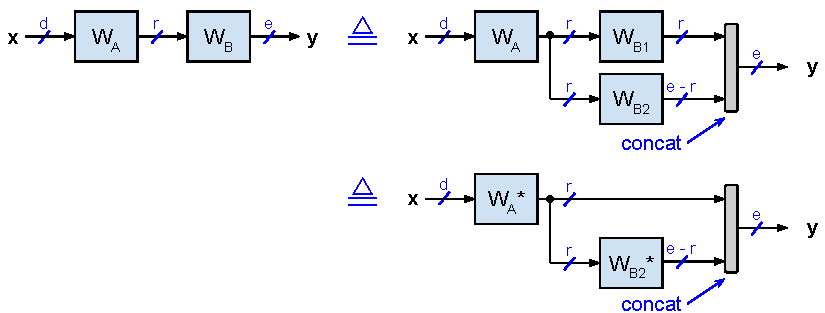
\includegraphics[scale=0.88]{../doc/fig/matShrink_fig1.pdf}
  \caption{Mathematically equivalent implementations of two back-to-back weight matrices $W_A$ and $W_B$ (left) with rank $r$, where $d > r$ and $e > r$, which reduces the total number of weights by $r^2$ (right).}
\label{fig1} \end{figure}

\section{Introduction}
The dominant cost of serving large transformer models is parameter count: it dictates memory footprint, memory bandwidth, and arithmetic throughput. A large body of work addresses this through \emph{approximate} compression---SVD-based low-rank factorization \citep{MoDeGPT,laser}, magnitude or structured pruning, and quantization---all of which trade accuracy for efficiency. A complementary and largely underexplored direction is \emph{exact} compression: identifying algebraic redundancies in the weight structure that can be eliminated without changing the function computed.

We observe that back-to-back linear layers---pairs of weight matrices applied sequentially with no nonlinearity between them---are ubiquitous in transformers and admit precisely such a redundancy. When $W_B \in \mathbb{R}^{r \times e}$ has full row rank $r$, any invertible $r \times r$ sub-block of $W_B$ can be absorbed into $W_A$ via an invertible change of basis on the shared inner dimension $r$, eliminating $r^2$ parameters while leaving the matrix product $W_A W_B$ unchanged. We call this procedure \textbf{MatShrink}.

MatShrink is complementary to approximate compression: it applies as a lossless post-processing step after SVD-based rank reduction, and is equally applicable to retrofitting existing models and to designing future architectures from scratch.

\paragraph{Contributions.}
\begin{enumerate}[topsep=2pt, itemsep=1pt]
  \item We state and prove MatShrink as a formal proposition and derive the closed-form weight savings (Section~\ref{sec:method}).
  \item We show that the attention dot-product is preserved under MatShrink applied to Q-K projections, even though the individual queries and keys change (Section~\ref{sec:mha}).
  \item We specialize MatShrink to MHA, MLA, GQA, and MQA, quantifying per-model savings and establishing the correct application order for MLA (Sections~\ref{sec:mha}--\ref{sec:gqa}).
  \item We identify the bf16 numerical instability, diagnose its root cause as ill-conditioned transformation matrices, and show that pivoted QR basis selection improves the numerical stability (Section~\ref{sec:precision}).
  \item We empirically validate all theoretical claims on four models across two attention variants (Section~\ref{sec:experiments}).
\end{enumerate}

\paragraph{Related work.}
Approximate weight compression schemes \citep{MoDeGPT,laser} use SVD or other low-rank approximations to reduce parameter counts at the cost of accuracy; MatShrink is exact and incurs no accuracy loss. Slim attention \citep{slimAttn} is the closest prior work, also using matrix inversion on V-O projections, but targeting \emph{KV-cache} size rather than static weight count. Weight fusion for the special case $e \leq r$ (absorbing two matrices into one) appears in \cite{remove,marko}; MatShrink strictly generalizes this to $e > r$, where full fusion is infeasible but $r^2$ weights can still be removed losslessly. ConvBN fusion \citep{convBN} is the convolutional analogue of MatShrink. Quantization-aware design \citep{smoothQuant} and weight sharing are orthogonal axes of compression that compose directly with MatShrink.

%\textbf{Related work.} Many weight compression schemes for transformers have been proposed such as \cite{MoDeGPT} and \cite{laser}. However, these schemes approximate the original weight matrices by using SVD (singular value decomposition) or other approximations. MatShrink on the other hand is not an approximation but an exact, mathematically equivalent optimization for back-to-back matrices. Furthermore, MatShrink is similar to slim attention \citep{slimAttn} in its use of matrix inversion to compute projections from each other.

\section{MatShrink: Formal Treatment} \label{sec:method}

\subsection{Setup and Core Proposition}

\begin{definition}[Back-to-back linear layer pair]
\label{def:b2b}
Let $W_A \in \mathbb{R}^{d \times r}$ and $W_B \in \mathbb{R}^{r \times e}$ with $d > r$ and $e > r$. A \emph{back-to-back linear layer pair} is the matrix product $W_A W_B$ with no nonlinearity between $W_A$ and $W_B$.
\end{definition}

\begin{proposition}[MatShrink]
\label{prop:matshrink}
Let $W_A \in \mathbb{R}^{d \times r}$ and $W_B \in \mathbb{R}^{r \times e}$ with $\rank(W_B) = r$. Partition $W_B = [W_{B1},\, W_{B2}]$ where $W_{B1} \in \mathbb{R}^{r \times r}$ is invertible and $W_{B2} \in \mathbb{R}^{r \times (e-r)}$. Define
$ W_A^* = W_A W_{B1}$ and $W_{B2}^* = W_{B1}^{-1} W_{B2}$, then:
\begin{equation}
  W_A W_B \;=\; W_A^* \bigl[I_r,\; W_{B2}^*\bigr],
  \label{eq:matshrink}
\end{equation}
where $I_r$ is the $r \times r$ identity matrix. The right-hand side stores $dr + r(e-r) = dr + re - r^2$ parameters, a reduction of $r^2$ over the original $dr + re$.
\end{proposition}

\begin{proof}
\begin{align*}
  W_A^* [I_r,\, W_{B2}^*]
  &= (W_A W_{B1}) [I_r,\, W_{B1}^{-1} W_{B2}] \\
  &= W_A \bigl[W_{B1} I_r,\; W_{B1} W_{B1}^{-1} W_{B2}\bigr] \\
  &= W_A [W_{B1},\, W_{B2}] = W_A W_B. \qedhere
\end{align*}
\end{proof}

Figure~\ref{fig1} illustrates Proposition~\ref{prop:matshrink} for a single pair.

\begin{remark}[Dual formulation]
\label{rem:dual}
An equivalent $r^2$ reduction is obtained by shrinking $W_A$ instead. Partition $W_A = [W_{A1};\, W_{A2}]$
with $W_{A1} \in \mathbb{R}^{r \times r}$ invertible, $W_{A2} \in \mathbb{R}^{(d-r) \times r}$.
Then $W_A W_B = \left[ W_{A1}; W_{A2} \right] W_B = \left[ I_r; W_{A2}^\ast \right] W_B^\ast$
where $W_B^\ast = W_{A1} W_B$ and $W_{A2}^\ast = W_{A2} W_{A1}^{-1}$, see Fig. \ref{fig2}.
This is the natural choice when it is preferable to preserve the structure of $W_B$.
\end{remark}

%\textbf{Alternative way.} Alternatively, we can split matrix $W_A$ into two submatrices
%$W_{A1}$ \eR{r}{r} and $W_{A2}$ such that $W_A = [W_{A1}; W_{A2}]$.
%We can then eliminate $W_{A1}$ as $W = \left[ W_{A1}; W_{A2} \right] W_B = \left[ I; W_{A2}^\ast \right] W_B^\ast$ with identity matrix $I$ \eR{r}{r} and where $W_B^\ast = W_{A1} W_B$ and $W_{A2}^\ast = W_{A2} W_{A1}^{-1}$, see Fig. \ref{fig2}. This also saves $r^2$ weights and $r^2$ multiply operations per token $x$.

\begin{figure}[h!] \centering
  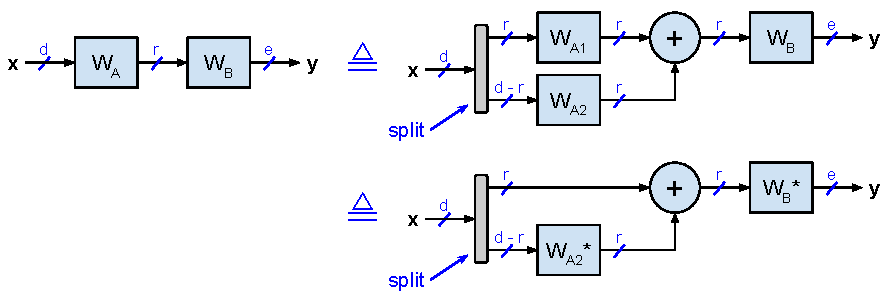
\includegraphics[scale=0.88]{../doc/fig/matShrink_fig2.pdf}
  \caption{Alternative formulation (Remark~\ref{rem:dual}): $r^2$ weights are eliminated from $W_A$ instead of $W_B$.}
  % TODO: \caption{Alternative way of shrinking $W_A$ instead of $W_B$}
\label{fig2} \end{figure}

%\paragraph{Weight savings.}\label{cor:savings}
%Under Proposition~\ref{prop:matshrink}, the parameter count decreases from $dr + re$ to $dr + re - r^2$, a multiplicative reduction factor of
%\[
%  \rho = 1 - \frac{r^2}{dr + re} = 1 - \frac{r}{d + e}.
%\]
%For the square case $d = e$: $\rho = 1 - r/(2d)$. Savings are maximized when $r \ll \min(d,e)$ and vanish when $d = e = r$.

%Inverting the submatrix $W_{B1}$ requires that this submatrix is invertible, which is often the case because it is extremely rare for large matrices to be non-invertible. In the rare case that $W_{B1}$ is non-invertible, we can first permute the columns of the original matrix $W_B$ such that the first $r$ columns of the permuted matrix form an invertible submatrix $W_{B1}$.

For completeness, if $e = r$, then the entire matrix $W_{B2}$ is eliminated. In general, if $e \leq r$, then the two matrices $W_A$ and $W_B$ can be fused into a single matrix $W^\ast = W_A \cdot W_B$ with only $d e$ weights (instead of $d r + r e$ weights for the original matrices $W_A$ and $W_B$). This type of weight fusion is utilized in \cite{remove, marko}.

\subsection{Algorithm}
Algorithm~\ref{alg:matshrink} is a complete, self-contained preprocessing procedure for retrofitting a pretrained model. Steps 1--4 are a one-time, per-layer cost; the forward pass (Step 5) requires no additional runtime modifications.

\begin{algorithm}[ht]
\caption{MatShrink: preprocessing a back-to-back layer pair}
\label{alg:matshrink}
\begin{algorithmic}[1]
\Require $W_A \in \mathbb{R}^{d \times r}$, $W_B \in \mathbb{R}^{r \times e}$ with $e > r$
\Ensure Compressed pair $(W_A^*, W_{B2}^*, P)$ computing the same function as $(W_A, W_B)$
\State \textbf{Pivot selection}: $(Q, R, P) \gets \mathrm{pQR}(W_B^\top)$; set $M \gets W_B[:, P[:r]]$ \Comment{Section~\ref{sec:precision}}
\State \textbf{Inversion}: $M^{-1} \gets $ fp64 LU factorization of $M$
\State \textbf{Absorb}: $W_A^* \gets W_A M$ \Comment{one-time $O(dr^2)$ cost}
\State \textbf{Reduce}: $W_{B2}^* \gets M^{-1} W_B[:, P[r:]]$ \Comment{eliminates $r \times r$ block $M$}
\State \textbf{Forward} (inference): $h \gets x W_A^*$; output$[:, P[:r]] \gets h$ (identity passthrough); output$[:, P[r:]] \gets h \cdot W_{B2}^*$
\end{algorithmic}
\end{algorithm}

%For two back-to-back weight matrices $W_A$ and $W_B$, Fig. \ref{fig1} illustrates how MatShrink reduces the size of $W_B$ in a mathematically equivalent way by using matrix inversion.
%Specifically, $W_A$ is a $d \times r$ matrix, $W_B$ is an $r \times e$ matrix with rank $r$, where $d > r$ and $e > r$. We can split $W_B$ into two submatrices $W_{B1}$ \eR{r}{r} and $W_{B2}$ such that $W_B = \left[ W_{B1}, W_{B2} \right]$. We can then eliminate $W_{B1}$ by merging it into $W_A$ as $W_A^\ast = W_A W_{B1}$ and by changing $W_{B2}$ to $W_{B2}^\ast = W_{B1}^{-1} W_{B2}$. This saves $r^2$ weights and $r^2$ multiply operations per token $x$. The following equation shows the mathematical identity of the modified back-to-back matrices, where $I$ is the $r \times r$ identity matrix:
%\begin{equation*}
%  W = W_A \cdot W_B \
%    = W_A \cdot [ W_{B1}, W_{B2} ] \
%    = W_A W_{B1} \cdot \left[ I, W_{B1}^{-1} W_{B2} \right] \
%    = W_A^\ast \cdot \left[ I, W_{B2}^\ast \right]
%\end{equation*}

\section{MatShrink for MHA Transformers}
\label{sec:mha}

\paragraph{V-O projections.}
In multi-head attention (MHA) \citep{vanilla}, the value (V) and output (O) projections for head $i$ form a back-to-back pair $W_{V,i} \in \mathbb{R}^{d \times r}$, $W_{O,i} \in \mathbb{R}^{r \times d}$, with no nonlinearity between them (Fig.~\ref{fig3}). Proposition~\ref{prop:matshrink} applies directly.

\begin{figure}[h!] \centering
  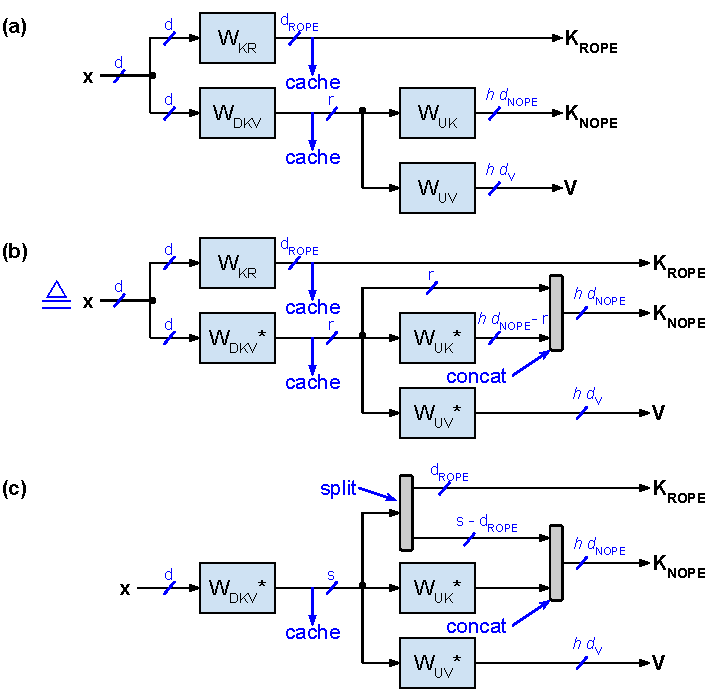
\includegraphics[scale=0.88]{../doc/fig/matShrink_fig3.pdf}
  \caption{MatShrink (Proposition~\ref{prop:matshrink}) applied to the V-O projection pair of a single attention head: (a) original; (b) compressed, eliminating $r^2 = d_k^2$ weights from $W_O$; (c) alternative formulation where $r^2$ weights are eliminated from $W_V$ rather than $W_o$.}
\label{fig3} \end{figure}

\paragraph{MHA V-O savings.}\label{prop:mha-vo}
For MHA with $h$ heads and model dimension $d = d_\text{model}$, each head has dimension $r = d_k = d/h$. Applying MatShrink to every head's V-O pair eliminates $r^2 = d^2/h^2$ weights per head and $d^2/h$ weights per layer in total---a fraction $1/(2h)$ of the $2d^2$ total V-O parameters.
%This follows directly from the weight savings formula with $e = d$ and $r = d/h$:
Savings per head $= r^2 = d^2/h^2$; summing over $h$ heads gives $d^2/h$. Table~\ref{tab1} shows the MHA V-O savings for representative models.

\begin{table}[h!] \centering
\caption{MHA weight savings from MatShrink (V-O projections). ``Savings'' is weights eliminated per layer; ``savings \%'' is relative to all V-O parameters ($2d^2$ per layer). The savings formula $d_k^2 h$ follows from the MHA V-O savings derivation in Section~\ref{sec:mha}.}
\begin{tabular}{lcccccc} \fline
  \thead[l]{Model} & \thead{$d$} & \thead{$d_k$} & \thead{$h$} & \thead{weights \\ $d \times (d_k h)$} & \thead{savings \\ $d_k^2 h$} & \thead{savings \\ \%} \\ \hline
  Whisper-tiny \cite{whisper}    & 384    & 64   & 6    & 147K   & 25K   & 17\% \\
  CodeGemma-7B \cite{codeGemma}  & 3,072  & 256  & 16   & 12.6M  & 1.0M  & 8\%  \\
  T5-3B \cite{T5}                & 1,024  & 128  & 32   & 4.2M   & 0.5M  & 12\% \\
  T5-11B \cite{T5}               & 1,024  & 128  & 128  & 16.8M  & 2.1M  & 13\% \\ \fline
\end{tabular} \label{tab1} \end{table}

\paragraph{Q-K projections.}
For models without RoPE and without QK-normalization (e.g., Whisper \cite{whisper}, T5 \cite{T5}), the query and key projections $W_{Q,i}, W_{K,i}$ form a back-to-back pair whose composition determines the attention logits.

\begin{figure}[h!] \centering
  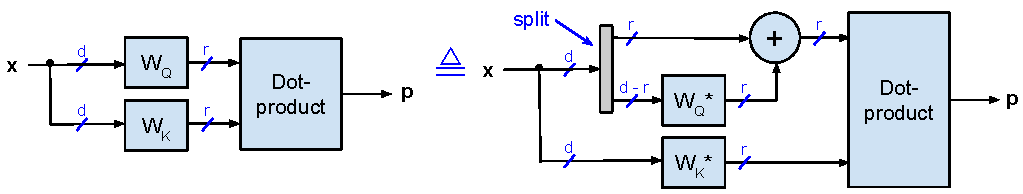
\includegraphics[scale=0.88]{../doc/fig/matShrink_fig5.pdf}
  \caption{MatShrink for Q-K projections (Section~\ref{sec:mha}) of a single attention head.
    Left: original Q and K projections and their dot-product $p$.
    Top right: equivalent implementation using MatShrink, which eliminates $r^2$ weights from $W_Q$.
    Bottom right: alternative implementation, which eliminates $r^2$ weights from $W_K$.}
%  \caption{Dual Q-K MatShrink: $r^2$ weights eliminated from $W_K$ (cf.\ Section~\ref{sec:mha} with $T = W_{K1}$).}
  % TODO: \caption{Alternative MatShrink implementation for Q and K projections of a single attention head. Left: original Q and K projections and their dot-product $p$. Right: equivalent implementation using MatShrink, which eliminates $r^2$ weights from $W_K$ (instead of $W_Q$).}
\label{fig5} \end{figure}

\paragraph{Q-K dot-product invariance under MatShrink.}\label{prop:qk}
MatShrink also applies to the query and key weight matrices $W_Q$ and $W_K$, with one twist: unlike V-O, the goal is not to compress a sequential product $W_Q W_K$, but to preserve the attention dot-product $Q K^\top = (x W_Q)(x W_K)^\top$. The key observation is that multiplying $W_Q$ by any invertible matrix $T$ and $W_K$ by $(T^{-1})^\top$ leaves every dot-product unchanged, since the two transformations cancel:
\[
  (x W_Q T) \left(x W_K (T^{-1})^\top \right)^\top = x W_Q T T^{-1} (x W_K)^\top = (x W_Q)(x W_K)^\top.
\]
Crucially, the transformed queries $Q^* = x W_Q T$ and keys $K^* = x W_K (T^{-1})^\top$ are individually different from the originals---yet their dot-product $Q^* {K^*}^\top$ is identical to $Q K^\top$ for every possible input. This means the attention scores, and therefore the model outputs, are completely unchanged.

\paragraph{Partial RoPE.}
Many modern models apply RoPE to only a fraction $\alpha \in (0,1)$ of $d_k$ (typically $\alpha = 1/2$ or less). The dot-product invariance result above applies to the non-RoPE portion of size $(1-\alpha)d_k$, yielding per-head savings of $(1-\alpha)^2 d_k^2$.

%Figure~\ref{fig6} shows the dual Q-K formulation eliminating weights from $W_K$ instead of $W_Q$.

%\textbf{MatShrink for transformers.} MatShrink reduces the number of weights for the following back-to-back weight matrices in transformer models:
%\begin{itemize}[topsep=-1pt]
%  \item The V (value) and O (output) projections for each attention-head, see Fig. \ref{fig3} and \ref{fig4}
%  \item The Q (query) and K (key) projections for each attention-head (without the RoPE portion), see Fig. \ref{fig5} and \ref{fig6}
%  \item The latent projections of MLA (multi-head latent attention), see Fig. \ref{fig7}(b)
%\end{itemize}

%\section{MatShrink for MHA transformers}

%\textbf{MatShrink for V and O projections.} Note that the value (V) and output (O) projections for each head $i$ of multi-head attention (MHA) are two back-to-back weight matrices $W_{V,i}$ and $W_{O,i}$ as illustrated in Fig. \ref{fig3} for a single attention head. Fig. \ref{fig3} shows how MatShrink eliminates $r^2$ weights from the original O projection weight matrix $W_O$. Alternatively, Fig. \ref{fig4} illustrates how the alternative MatShrink scheme from Fig. \ref{fig2} can eliminate $r^2$ weights from the original V projection (instead of the O projection).

%For MHA, we can apply the MatShrink scheme to each head. Specifically:
%\begin{itemize}[topsep=-1pt]
%  \item For the vanilla MHA with $h$ heads, each head has dimension $d_k = d / h$, and $d = d_\text{model}$.
%  \item So for the dimensions $r$ and $e$ of Fig. \ref{fig1}, we have  $r = d / h$ and $e = d$.
%  \item This saves $r^2 = d^2 / h^2$ weights for each head, so $d^2 / h$ weights in total.
%  \item Note that for single-head attention (where $h = 1$), we can save $2 d^2$ weights: Specifically, we can merge the V and O weight matrices into a single $d \times d$ matrix; and the Q and K weight matrices into a single $d \times d$ matrix (if there is no RoPE).
%\end{itemize}

%Table \ref{tab1} lists the configurations of various MHA transformer models, the number of weights for their attention projections, and the weight savings provided by MatShrink.
%\begin{table}[h!] \centering
%\caption{Weight savings for MHA transformer models using MatShrink}
%\begin{tabular}{lcccccc} \fline
%  \thead[l]{Model} & \thead{$d$} & \thead{$d_k$} & \thead{$h$} & \thead{weights \\ $d \times (d_k h)$} & \thead{savings \\ $d_k^2 h$} & \thead{savings \\ \%} \\ \hline
%  Whisper-tiny \cite{whisper}    & 384    & 64   & 6    & 147K   & 25K   & 17\% \\
%  CodeGemma-7B \cite{codeGemma}  & 3,072  & 256  & 16   & 12.6M  & 1.0M  & 8\%  \\
%  T5-3B \cite{T5}                & 1,024  & 128  & 32   & 4.2M   & 0.5M  & 12\% \\
%  T5-11B \cite{T5}               & 1,024  & 128  & 128  & 16.8M  & 2.1M  & 13\% \\ \fline
%\end{tabular} \label{tab1} \end{table}

%\textbf{MatShrink for Q and K projections.} For models that don’t use RoPE (such as Whisper \cite{whisper} and T5 models \cite{T5}), the query (Q) and key (K) projections for each head $i$ of MHA are two back-to-back weight matrices $W_{Q,i}$ and $W_{K,i}$ as illustrated in Fig. \ref{fig5} for a single attention head.

%Fig. \ref{fig5} shows how MatShrink eliminates $r^2$ weights from the original Q weight matrix $W_Q$. Note that the queries $Q^\ast$ and keys $K^\ast$ generated by the modified linear layers $W_Q^\ast$ and $W_K^\ast$ are not identical to the original queries $Q$ and keys $K$, but their dot-products $p$ are identical, i.e. $p = Q \cdot K = Q^\ast \cdot K^\ast$.

%For many models that use RoPE, we can also apply this trick as follows: Many modern transformer models use partial RoPE, which applies RoPE to only a portion of the head-dimension $d_k = d / h$, usually only to one half of $d_k$. So in this case $r = d_k / 2 = d / (2h)$, which saves only $r^2 = d^2 / (4h^2)$ weights for each head, so $d^2 / (4h)$ weights in total.

%For completeness, Fig. \ref{fig6} illustrates an alternative implementation of MatShrink that removes $r^2$ weights from $W_K$ instead of $W_Q$.

\section{MatShrink for GQA and MQA} \label{sec:gqa}
\paragraph{GQA and MQA.}\label{cor:gqa}
For grouped-query attention \citep{GQA} with grouping factor $g = n_\text{heads}/n_\text{KV-heads}$, MatShrink applies per KV-group. The per-group V-O savings are $d_k^2$ (from the MHA savings derivation above); the savings per query head are reduced by factor $g$ relative to MHA. For MQA ($g = n_\text{heads}$), the single shared V-O pair still yields $d_k^2$ savings in absolute terms.

%\section{MatShrink for GQA and MQA}
%MatShrink is not limited to MHA and MLA only. It’s also applicable to GQA (grouped query attention) and MQA (multi-query attention). However, the savings are smaller than for MHA and MLA. Specifically, the savings are reduced by a factor $g$, where $g$ is the number of queries that are shared among a single KV-pair, or in other words $g = n_\text{heads} / n_\text{KV-heads}$ (where $n_\text{heads}$ is the number of query-heads, and $n_\text{KV-heads}$ is the number of KV-heads).

\section{MatShrink for MLA Transformers} \label{sec:mla}
We follow the notation of \citet{deepseek-v2}. $r_\text{Q}$: Q-latent rank; $\WW{DQ}$: Q down-projection; $\WW{UQ}$: Q NoPE up-projection; $\WW{QR}$: Q RoPE up-projection; $r_\text{KV}$: KV-latent rank; $\WW{DKV}$: KV down-projection; $\WW{UK}$, $\WW{UV}$: K and V NoPE up-projections; $\WW{KR}$: K RoPE projection. Table~\ref{tab2} gives configurations of representative MLA models.

% shortcuts (only letters allowed in macro names)
\def\dsRone     {\href{https://huggingface.co/deepseek-ai/DeepSeek-R1}         {DeepSeek-R1}}
\def\pplRone    {\href{https://huggingface.co/perplexity-ai/r1-1776}           {Perplexity R1-1776}}
\def\dsVthree   {\href{https://huggingface.co/deepseek-ai/DeepSeek-V3}         {V3}}
\def\misLarge   {\href{https://huggingface.co/mistralai/Mistral-Large-3-675B-Base-2512} {Mistral Large 3 675B}}
\def\dsVtwoFive {\href{https://huggingface.co/deepseek-ai/DeepSeek-V2.5}       {DeepSeek-V2.5}}
\def\dsVtwoL    {\href{https://huggingface.co/deepseek-ai/DeepSeek-V2-Lite}    {DeepSeek-V2-lite}}
\def\dsVLtwoS   {\href{https://huggingface.co/deepseek-ai/deepseek-vl2-small}  {VL2-small }}
\def\MiniCPM    {\href{https://huggingface.co/openbmb/MiniCPM3-4B}             {OpenBMB MiniCPM3-4B }}

\begin{table}[h!] \centering
\caption{Configurations of representative MLA transformer models.}
\begin{tabular}{lcccccccc} \fline
  \thead[l]{Model} & \thead{Params} & $d$ & $r_\text{Q}$ & $r_\text{KV}$ & $h$ & $d_\text{NOPE}$ & $d_\text{ROPE}$ \\ \hline
  \pplRone, \dsRone, \dsVthree           & 685B  & 7,168  & 1,536  & 512  & 128  & 128  & 64 \\
  \misLarge                              & 675B  & 7,168  & 1,536  & 512  & 128  & 128  & 64 \\
  \dsVtwoFive                            & 236B  & 5,120  & 1,536  & 512  & 128  & 128  & 64 \\
  \dsVtwoL, \dsVLtwoS \cite{deepseek-v2} & 16B   & 2,048  & N/A    & 512  & 16   & 128  & 64 \\
  \MiniCPM \cite{miniCPMv2}              & 4B    & 2,560  & 768    & 256  & 40   & 64   & 32 \\ \fline
\end{tabular} \label{tab2} \end{table}

\paragraph{MLA MatShrink application order.}\label{prop:mla-order}
MatShrink can be applied to MLA attention weights in the following four-step sequence, where each step is a valid application of Proposition~\ref{prop:matshrink} or the Q-K invariance result above:
\begin{enumerate}[topsep=2pt, itemsep=0pt]
  \item Apply MatShrink to the per-head V-O pairs $(\WW{UV,i}, \WW{O,i})$: eliminates $h \cdot d_\text{NOPE}^2$ weights.
  \item Apply the Q-K dot-product invariance to the NoPE portion of the per-head Q-K pairs: eliminates $h \cdot d_\text{NOPE}^2$ weights while preserving attention logits.
  \item Apply MatShrink to the Q-latent pair $(\WW{DQ}, \WW{UQ}^*)$, where $\WW{UQ}^*$ is the result of step~2. \emph{Must follow step~2.}
  \item Apply MatShrink to the KV-latent pair $(\WW{DKV}, [\WW{UK}; \WW{UV}^*])$, where $\WW{UV}^*$ is the result of step~1. \emph{Must follow step~1.}
\end{enumerate}
Steps 1 and 2 act on disjoint weight pairs and are independent. After step~2, $\WW{UQ}$ is modified to $\WW{UQ}^*$, but the composite map $\WW{DQ} \WW{UQ}^*$ is identical to $\WW{DQ} \WW{UQ}$ (by the Q-K dot-product invariance above); hence step~3 is a valid application of Proposition~\ref{prop:matshrink} to $(\WW{DQ}, \WW{UQ}^*)$. Step~4 is analogous.

However, many MLA models deploy latent normalization by having an RMSNorm layer in-between each pair of down- and up-projections. This normalization prevents applying MatShrink to the Q-latent pair and KV-latent pair (steps 3 and 4).

%\paragraph{Concrete savings for DeepSeek-R1/V3.}
%For the 685B-class models ($d=7168$, $r_\text{KV}=512$, $r_\text{Q}=1536$, $h=128$, $d_\text{NOPE}=128$, 61 layers), the four steps of the application order above eliminate per layer: step~1: $128 \times 128^2 = 2{,}097{,}152$ weights; step~2: $2{,}097{,}152$ weights; step~3: $1536^2 = 2{,}359{,}296$ weights; step~4: $512^2 = 262{,}144$ weights. Total: $\approx 6.8\text{M}$ weights per layer, or $\approx \mathbf{414M}$ parameters eliminated across all 61 attention layers, with zero accuracy cost.

%\section{MatShrink for MLA transformers}
%Table \ref{tab2} shows the configurations of various transformer models with MLA. We are using the following parameter names similar to \citep{deepseek-v2}:
%\begin{itemize}[topsep=-1pt]
%  \item For Q (query):
%  \begin{itemize}[topsep=-1pt]
%    \item $r_\text{Q}$: rank of Q-latent projection
%    \item $\WW{DQ}$: down-projection for Q
%    \item $\WW{UQ}$: up-projection for Q-part without RoPE (aka NoPE)
%    \item $\WW{QR}$: up-projection for Q-part with RoPE
%  \end{itemize}
%  \item For KV (key-value):
%  \begin{itemize}[topsep=-1pt]
%    \item $r_\text{KV}$: rank of KV-latent projection
%    \item $\WW{KR}$: projection for K-part with RoPE (has its own cache, used for all queries as MQA)
%    \item $\WW{DKV}$: down-projection for KV
%    \item $\WW{UK}$: up-projection for K-part without RoPE (aka NoPE)
%    \item $\WW{UV}$: up-projection for V
%  \end{itemize}
%\end{itemize}

% BEFORE with column h * d_NOPE
%  \thead[l]{Model} & \thead{Params} & $d$ & $r_\text{Q}$ & $r_\text{KV}$ & $h$ & $d_\text{NOPE}$ & $h \cdot d_\text{NOPE}$ & $d_\text{ROPE}$ \\ \hline
%  Perplexity \pplRone, \dsRone, and \dsVthree  & 685B  & 7,168  & 1,536  & 512  & 128  & 128  & 16,384  & 64 \\
%  \dsVtwoFive                                  & 236B  & 5,120  & 1,536  & 512  & 128  & 128  & 16,384  & 64 \\
%  \dsVtwoL, \dsVLtwoS                          & 16B   & 2,048  & N/A    & 512  & 16   & 128  & 2,048   & 64 \\
%  OpenBMB \MiniCPM                             & 4B    & 2,560  & 768    & 256  & 40   & 64   & 2,560   & 32 \\ \fline

%DeepSeek's MLA (multi-head latent attention) scheme \citep{deepseek-v2} has two latent projections, one for Q (queries) and one for KV (keys and values). We can apply MatShrink to each of them:
%\begin{itemize}[topsep=-1pt]
%  \item The Q-latent projection and query (Q) projections are two back-to-back weight matrices $\WW{DQ}$ and $\WW{UQ}$.
%  \item The KV-latent projection and key/value (KV) projections are two back-to-back weight matrices $\WW{DKV}$ and the union of $\WW{UK}$ and $\WW{UV}$.
%\end{itemize}

%We can also apply MatShrink to each V-O head and the non-RoPE portion of the Q-K heads. Specifically, we can apply the MatShrink to the MLA weight matrices in the following order:
%\begin{enumerate}[topsep=-1pt, itemsep=-1pt]
%  \item Apply MatShrink to the V-O weight matrices.
%  \item Apply MatShrink to the NoPE portion (i.e. the non-RoPE portion) of the Q-K weight matrices.
%  \item Apply MatShrink to the Q-latent projections. This step must be done after applying MatShrink to the Q-K weights.
%  \item Apply MatShrink to the KV-latent projections. This step must be done after applying MatShrink to the V-O weights.
%\end{enumerate}

%Applying MatShrink to the KV-latent projections not only reduces weight matrices and corresponding compute, it can also reduce the compute complexity as follows, where $r_\text{KV}$ is the rank of the KV-latent projections.
%\begin{itemize}[topsep=-1pt]
%  \item Option 1: Use the $r_\text{KV}$ neurons that don’t require a weight matrix as keys. The number of those keys is $r_\text{KV} / d_\text{NOPE}$. Then these keys can be directly used for the softmax arguments, which saves some computation complexity.
%  \item Option 2: Use the $r_\text{KV}$ neurons as values (instead of keys). Then these values can be directly multiplied with the softmax scores, which saves some compute complexity.
%\end{itemize}

%TODO: details the savings, perhaps with a new table

%\section{Simplified MLA} \label{sec:simplified-mla}
%\begin{figure}[h!] \centering
%  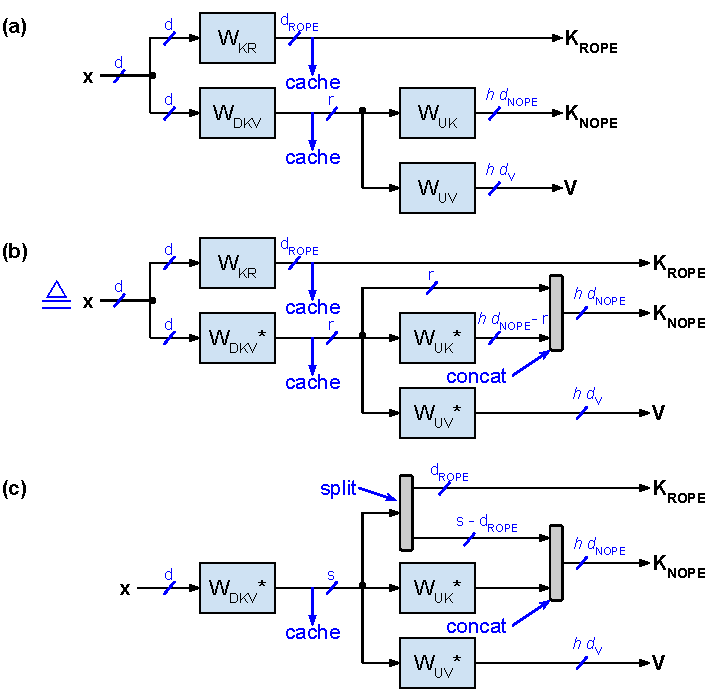
\includegraphics[scale=0.88]{../doc/fig/matShrink_fig7.pdf}
%  \caption{K-V projections for MLA: (a) original \citep{deepseek-v2}; (b) MatShrink-optimized (application order above, step~4); (c) proposed simplified MLA (Section~\ref{sec:simplified-mla}).}
  % TODO: \caption{K and V projections for MLA. (a) original version; (b) equivalent version optimized by MatShrink; (c) proposed simplification}
%\label{fig7} \end{figure}

%\paragraph{Simplified MLA.}\label{prop:simplified-mla}
%Standard MLA uses a dedicated $d_\text{ROPE}$-dimensional projection $\WW{KR}$ with its own per-token cache. We propose sourcing the RoPE key channels directly from the unified latent cache of dimension $s \in [r_\text{KV},\; r_\text{KV} + d_\text{ROPE}]$, eliminating $\WW{KR}$ and its separate cache. The trade-off is:
%\begin{itemize}[topsep=2pt, itemsep=0pt]
%  \item $s > r_\text{KV}$: higher effective KV rank, improved expressiveness, unified (larger) cache.
%  \item $s = r_\text{KV}$: unchanged total cache size; $d_\text{ROPE}$ latent channels are repurposed for RoPE keys.
%\end{itemize}
%In both cases, $\WW{KR} \in \mathbb{R}^{d \times d_\text{ROPE}}$ is eliminated, saving $d \cdot d_\text{ROPE}$ parameters per layer. For DeepSeek-R1/V3 ($d=7168$, $d_\text{ROPE}=64$, 61 layers): $\approx \mathbf{28M}$ additional parameters eliminated.

%This simplification is not mathematically equivalent to standard MLA and must be trained from scratch, but it offers a cleaner architectural design for future models by unifying the KV-cache into a single latent space.

%\section{Simplified MLA}
%In this section we propose a simplification for DeepSeek’s MLA (multi-head latent attention).

%Fig. \ref{fig7} shows the K and V projections of MLA and the proposed simplification:
%\begin{itemize}[topsep=-1pt]
%  \item Fig. \ref{fig7}(a) shows the MLA projections for K (keys) and V (values). Note that a single $d_\text{ROPE}$ head is shared among all query-heads, where $d_\text{ROPE} = 64$ or $32$ usually.
%  \item Fig. \ref{fig7}(b) shows the mathematically equivalent version with MatShrink applied to the weight matrices $\WW{DKV}$ and $\WW{UK}$.
%  \item Fig. \ref{fig7}(c) shows the proposed simplified MLA scheme where the $d_\text{ROPE}$ units (or channels) are sourced directly from the latent cache, instead of having a separate cache and $\WW{KR}$ for the $d_\text{ROPE}$ units:
%  \begin{itemize}[topsep=-1pt]
%    \item Note that this simplified scheme is not mathematically identical to the standard MLA scheme shown in Fig. \ref{fig7}(a).
%    \item The rank $s$ of the simplified scheme could be larger than $r$ (e.g. $s = r + d_\text{ROPE}$) or slightly lower than this (e.g. $s = r$).
%    \item Advantages include: If $s > r$, then there is more usable rank for the keys and values. So the cached latent space is better utilized. And if $s < r + d_\text{ROPE}$ then the total cache size is reduced.
%  \end{itemize}
%\end{itemize}

%This simplification enhances MLA by directly leveraging the latent cache for RoPE components, potentially increasing effective rank and optimizing cache utilization. In DeepSeek-V2, standard MLA already reduces KV cache by compressing into latent vectors, but our proposal further streamlines this by eliminating separate RoPE projections, leading to additional memory savings especially for long-sequence inference.

\section{MatShrink Combined with SVD-Based Compression}
\paragraph{Composability with low-rank approximation.}\label{prop:svd}
Let $W \approx \hat{W}_A \hat{W}_B$ be a rank-$r$ approximation of $W \in \mathbb{R}^{d \times e}$ (e.g., from truncated SVD). Since Proposition~\ref{prop:matshrink} requires only that $\hat{W}_A \in \mathbb{R}^{d \times r}$, $\hat{W}_B \in \mathbb{R}^{r \times e}$, and $\rank(\hat{W}_B) = r$---conditions satisfied by any full-rank SVD truncation---MatShrink applies directly to $(\hat{W}_A, \hat{W}_B)$, eliminating an additional $r^2$ parameters while computing $\hat{W}_A \hat{W}_B$ exactly and leaving the approximation gap $\|W - \hat{W}_A \hat{W}_B\|$ unchanged.

%\section{MatShrink for SVD}
%Approximate weight compression schemes such as \cite{laser} and \cite{MoDeGPT} use SVD (singular value decomposition) to reduce the ranks of weight matrices, and thus reduce weights. This is applicable for example for the large weight matrices of the transformer’s FFN (feedforward networks). The SVD decomposition factorizes the original matrix $W$ \eR{d}{e} into two matrices $W_A$ and $W_B$ where $r$ is the compressed rank. After performing SVD and compressing the rank by a certain percentage, we can then eliminate $r^2$ weights using our MatShrink scheme. Note that reducing the rank by a certain percentage is not an exact implementation of the original matrix $W$ but an approximation.

\section{Numerical Stability: Pivoted QR Basis Selection} \label{sec:precision}
MatShrink requires inverting a chosen $r \times r$ sub-block $M$ of $W_B$; any invertible choice gives the same mathematical result. In practice, however, the choice matters when weights are stored in bf16 or lower precision: if $M$ is nearly singular, $M^{-1}$ contains very large entries that amplify bf16 rounding errors in the compressed weights. With the naive choice of the first $r$ columns of $W_B$, this can cause perplexity to diverge (Table~\ref{tab:matshrink-bf16}). Under fp32 the problem does not arise.

\paragraph{Fix: pivoted QR column selection.}\label{prop:pqr}
We select $M$ using pivoted QR decomposition, which greedily picks the $r$ columns of $W_B$ that carry the most independent information---producing an $M$ that is as far from singular as possible:
\[
  (Q, R, P) \gets \mathrm{pQR}(W_B), \qquad M \gets W_B[:, P[:r]].
\]
In practice this is a one-liner: \texttt{scipy.linalg.qr(W\_B.T, pivoting=True)}. As Table~\ref{tab:matshrink-bf16} shows, this reduces bf16 regressions to within $\pm 0.05$ perplexity points of the source model's bf16 baseline across all four tested models.

\section{Experiments} \label{sec:experiments}
We validate MatShrink's core claim of mathematical equivalence empirically on four models spanning both attention variants covered by the paper and two head dimension: SmolLM2-135M \citep{smollm}, a 30-layer decoder-only transformer with GQA ($n_\text{heads} = 9$, $n_\text{KV} = 3$, $d_\text{head} = 64$); GPT-2-124M \citep{gpt2}, a 12-layer MHA transformer ($n_\text{heads} = 12$, $d_\text{head} = 64$); and Gemma-3 \citep{gemma3} at the 1B (text-only) and 4B (multimodal, text-backbone-only) sizes, both with $d_\text{head} = 256$, the regime where MatShrink's per-head $r^2$ savings accumulate most (Table \ref{tab1}). All experiments run on a single NVIDIA A100 GPU and evaluate perplexity on the full WikiText-2 raw test split using non-overlapping context-length windows.

\subsection{Correctness under fp32}
We apply V-O MatShrink to every attention layer. For each KV group (GQA) or each attention head (MHA), we select the transformation matrix $M$ and compute $M^{-1}$ in double precision. Reconstruction error at the identity block is $\mathcal{O}(10^{-14})$ on every model (fp64 machine precision).

With shrunk weights stored in fp32, baseline and MatShrink perplexities match exactly on all four models (Table \ref{tab:matshrink-correctness}), confirming that the transformation is mathematically equivalent and that inversion-induced numerical error is negligible at single precision.

\begin{table}[h!] \centering
\caption{WikiText-2 perplexity before and after V-O MatShrink, fp32 storage, full test split.}
\label{tab:matshrink-correctness}
\begin{tabular}{l r r r}
\hline
Model & Source & MatShrink & $\Delta$ \\
\hline
GPT-2-124M (MHA)     & 29.9394 & 29.9394 & 0.0000 \\
SmolLM2-135M (GQA)   & 15.4629 & 15.4629 & 0.0000 \\
Gemma-3-1B (GQA)     & 14.1839 & 14.1838 & $-0.0001$ \\
Gemma-3-4B (GQA)     & 10.7664 & 10.7664 & 0.0000 \\
\hline
\end{tabular}
\end{table}

\subsection{Numerical precision at bf16 and the role of basis choice on the shared inner dimension}
\label{sec:matshrink-precision}

\textbf{Problem.} The precision issue is specific to bf16 storage. Under fp16 the identity-$M$ variant is already essentially lossless (the fp16 rows of Table \ref{tab:matshrink-bf16} show absolute regressions of only $+0.01$ ppl on SmolLM2-135M and $+0.06$ ppl on GPT-2-124M, both within benchmark noise); fp16's 10-bit mantissa carries enough precision to absorb the rewritten-weight magnitudes. bf16 trades 3 mantissa bits (10$\to$7) for 3 additional exponent bits (5$\to$8); it is the reduced mantissa that bites here. With the naive choice of $M$ (the leading $r \times r$ sub-block of the target $W_O$ slice), bf16 perplexity degrades substantially, and the degradation grows with head dimension: on $d_\text{head} = 64$ models the absolute ppl regression is $+1.51$ on SmolLM2-135M and $+18.94$ on GPT-2-124M; on $d_\text{head} = 256$ Gemma 3 it is $+25.29$ on the 1B variant (a qualitatively broken model) and $+8.98$ on the 4B variant. The root cause is that $M^{-1}$ amplifies bf16 rounding error when $M$ is ill-conditioned: the condition number of the naive $M$ has a heavy tail on every model (up to $\kappa = 1.67 \times 10^5$ on GPT-2, $\kappa = 1.58 \times 10^5$ on Gemma-3-4B), and the entries of $W_V^\ast = W_V M$ and $W_{O_2}^\ast = M^{-1} W_{O_2}$ then span a range that bf16's 8-bit mantissa cannot faithfully represent. Error compounds across layers.

\textbf{Fix: change of basis on the shared inner dimension, realized by pivoted QR.} The two back-to-back matrices $W_V$ and $W_O$ meet along a shared $r$-dimensional axis (the head dimension, which is the inner dimension of the composite product). Applying any invertible change of basis $T \in \mathbb{R}^{r \times r}$ to this shared axis as $W_V \mapsto W_V T$ and $W_O \mapsto T^{-1} W_O$ leaves the composite $W_V W_O$ unchanged, so the model's output at every token position is preserved exactly. What $T$ does change is \emph{which} $r \times r$ sub-block of $W_O$ ends up in MatShrink's leading position and therefore gets inverted as $M$. A pure permutation of this shared axis is the orthogonal special case, and because orthogonal transformations preserve singular values it leaves $\text{cond}(M)$ unchanged; a general invertible $T$ reduces $\text{cond}(M)$ by one to three orders of magnitude on the models we test.

We select the change of basis implicitly by picking $M$ directly as the best-conditioned $r \times r$ sub-block of $W_O$, identified by rank-revealing (pivoted) QR decomposition of $W_O$:
\begin{equation*}
    (Q, R, P) \gets \mathrm{QR}(W_O,\; \text{pivoting}=\mathtt{True}), \qquad M \gets W_O\bigl[\,:,\; P[:r]\,\bigr],
\end{equation*}
which, by classical argument, selects the $r$ columns of $W_O$ forming the best-conditioned leading block available. The corresponding explicit change of basis would be $T = M \cdot M_0^{-1}$ with $M_0 = W_O[:,:r]$ the naive leading sub-block; running vanilla MatShrink on $(W_V T, T^{-1} W_O)$ produces the same $W_V^\ast$ and $W_O^\ast$ as picking $M$ directly, and the direct approach is the one-line shortcut used in the implementation. Alternative choices (column-$L_2$ sort, random sub-block sampling) are valid changes of basis as well and give partial improvements; pivoted QR is used because its conditioning guarantee is the strongest and because it is a one-line call in \texttt{scipy.linalg}. The resulting model is mathematically identical to the naive variant at fp32, stores the same number of weights, and loads in stock HuggingFace Transformers and vLLM without modification; the identity block simply lives at the column indices $P[:r]$ rather than at the contiguous prefix $[0, r)$.

\textbf{Result.} Pivoted QR reduces condition numbers by 1--3 orders of magnitude at the tail (Table \ref{tab:matshrink-cond}) and collapses the bf16 perplexity regression to within $\pm 0.05$ of the source model's bf16 perplexity on every tested configuration (Table \ref{tab:matshrink-bf16}). The fp32 perplexities are unchanged, as required by the mathematical invariance of the transformation.

\begin{table}[h!] \centering
\caption{Distribution of $\text{cond}(M)$ across all (layer, head/KV-group) pairs. Pivoted QR reduces the tail by roughly two orders of magnitude at $d_\text{head} = 64$ and by two to three orders at $d_\text{head} = 256$, where the naive tail is largest.}
\label{tab:matshrink-cond}
\begin{tabular}{l l r r r}
\hline
Model & Strategy & median $\kappa$ & 95th pct.\ $\kappa$ & max $\kappa$ \\
\hline
GPT-2-124M ($d_\text{head}{=}64$)   & identity & $255$     & $3.4 \times 10^3$ & $1.67 \times 10^5$ \\
                                    & pivoted  & $37$      & $118$             & $404$ \\
\hline
SmolLM2-135M ($d_\text{head}{=}64$) & identity & $436$     & $4.9 \times 10^3$ & $9.87 \times 10^3$ \\
                                    & pivoted  & $26$      & $86$              & $104$ \\
\hline
Gemma-3-1B ($d_\text{head}{=}256$)  & identity & $4.4 \times 10^3$ & $1.7 \times 10^4$ & $9.91 \times 10^4$ \\
                                    & pivoted  & $218$     & $563$             & $702$ \\
\hline
Gemma-3-4B ($d_\text{head}{=}256$)  & identity & $2.6 \times 10^3$ & $2.4 \times 10^4$ & $1.58 \times 10^5$ \\
                                    & pivoted  & $156$     & $570$             & $5.4 \times 10^3$ \\
\hline
\end{tabular}
\end{table}

\begin{table}[h!] \centering
\caption{WikiText-2 perplexity on full test split, with pivoted-QR $M$-selection vs.\ naive identity-slice $M$-selection. fp32 is mathematically invariant (identical to four decimal places). Under bf16, pivoted-QR closes the gap to the source model from as large as $+25.29$ absolute (Gemma-3-1B identity-$M$) to within $\pm 0.05$ on every model. Gemma 3 does not support fp16 inference on the source model (dynamic-range overflow), so only fp32 and bf16 are reported for those rows.}
\label{tab:matshrink-bf16}
\begin{tabular}{l l r r r}
\hline
Model & Precision & Source & Identity-$M$ & Pivoted-$M$ \\
\hline
GPT-2-124M   & fp32 & $29.9394$ & $29.9394$ & $29.9394$ \\
             & fp16 & $29.9482$ & $30.0038$ & $29.9467$ \\
             & bf16 & $30.2090$ & $49.1541$ & $\mathbf{30.1928}$ \\
\hline
SmolLM2-135M & fp32 & $15.4629$ & $15.4629$ & $15.4629$ \\
             & fp16 & $15.4634$ & $15.4775$ & $15.4634$ \\
             & bf16 & $15.4750$ & $16.9885$ & $\mathbf{15.4787}$ \\
\hline
Gemma-3-1B   & fp32 & $14.1839$ & $14.1838$ & $14.1839$ \\
             & bf16 & $14.1932$ & $39.4825$ & $\mathbf{14.1520}$ \\
\hline
Gemma-3-4B   & fp32 & $10.7664$ & $10.7664$ & $10.7664$ \\
             & bf16 & $10.7877$ & $19.7706$ & $\mathbf{10.8055}$ \\
\hline
\end{tabular}
\end{table}

\subsection{vLLM compatibility}

Because MatShrink in explicit-identity mode produces a standard checkpoint (identical tensor shapes and key names as the source), the shrunk model loads in vLLM \citep{vLLM} without modification to the runtime or model code. We verify end-to-end inference on SmolLM2-135M by running deterministic greedy generation before and after MatShrink; both produce coherent continuations from held-out prompts. The pivoted-QR variant is equivalent in this respect: the identity block lives at non-contiguous column indices, but every tensor retains its original shape and name, so no loader changes are required.

Because the identity blocks are stored as dense tensors, the runtime performs redundant matmuls and throughput is unchanged; realizing the compute savings implied by the identity structure requires runtime support, which we leave to future work.

\textbf{Note on further quantization.} A separate consequence of pivoted-QR selection is that $W_V^\ast$ and $W_O^\ast$ retain the magnitude range of the source $W_V$ and $W_O$ (since a well-conditioned $M^{-1}$ does not inflate entries), whereas the naive identity-$M$ variant produces rewritten weights with inflated magnitudes that track $\kappa(M)$. Downstream 8-bit or 4-bit weight quantization, which depends on a bounded weight distribution, should therefore compose more gracefully with pivoted-QR MatShrink than with the identity variant. Systematic evaluation of MatShrink plus quantization is left to future work.

\section{Conclusion}
We presented MatShrink, a theoretically grounded, empirically validated framework for losslessly eliminating $r^2$ parameters from any pair of consecutive linear layers. The core result (Proposition~\ref{prop:matshrink}) is an elementary change-of-basis identity; the pivoted QR analysis (Section~\ref{sec:precision}) establishes the numerically optimal choice of sub-block. Specializations to MHA, MLA, GQA, MQA (Sections~\ref{sec:mha}--\ref{sec:gqa}) quantify savings of 8--17\% of attention parameters for MHA.
Experiments on four models confirm exact fp32 equivalence and near-exact bf16 equivalence, with compressed checkpoints loading in production inference engines without modification.

\paragraph{Limitations and future work.}
The weight savings currently do not yield proportional throughput improvements, since identity blocks are stored and multiplied as dense tensors; realizing the compute reduction requires structured-sparse runtime support.
When pivoted QR is used, the column permutation must also be stored and applied at inference time (or folded into subsequent layers if possible); finding compact representations of this permutation and efficient kernel-level implementations is an additional open problem.
Beyond post-training compression, future models could adopt MatShrink's reduced weight structures from the outset, training directly on the smaller parameterization and achieving better parameter efficiency from scratch.
Extending empirical validation to MLA models, evaluating composition with post-training quantization (Section~\ref{sec:precision}), integrating MatShrink-aware kernels into production engines (llama.cpp \citep{llama-cpp}, SGLang \citep{sglang}) are natural directions for future work.

%\section*{Acknowledgments}
%We would like to thank TBD for helpful feedback on this work.

\bibliographystyle{unsrtnat}
\bibliography{references}

\newpage
\input{matShrink_checklist.tex}

\end{document}
